\documentclass[11pt,twoside,a4paper]{article}
% http://www-h.eng.cam.ac.uk/help/tpl/textprocessing/latex_maths+pix/node6.html symboles de math
% http://fr.wikibooks.org/wiki/Programmation_LaTeX Programmation latex (wikibook)
%=========================== En-Tete =================================
%--- Insertion de paquetages (optionnel) ---
\usepackage[french]{babel}   % pour dire que le texte est en fran{\'e}ais
\usepackage{a4}	             % pour la taille   
\usepackage[T1]{fontenc}     % pour les font postscript
\usepackage{epsfig}          % pour gerer les images
%\usepackage{psfig}
\usepackage{amsmath, amsthm} % tres bon mode mathematique
\usepackage{amsfonts,amssymb}% permet la definition des ensembles
\usepackage{float}           % pour le placement des figure
\usepackage{verbatim}

\usepackage{longtable} % pour les tableaux de plusieurs pages

\usepackage[table]{xcolor} % couleur de fond des cellules de tableaux

\usepackage{lastpage}

% \usepackage[top=1.5cm, bottom=1.5cm, left=1.5cm, right=1.5cm]{geometry}
% gauche, haut, droite, bas, entete, ente2txt, pied, txt2pied
\usepackage{vmargin}
\setmarginsrb{1.0cm}{1.0cm}{1.0cm}{1.0cm}{15pt}{3pt}{90pt}{3pt}

\usepackage{lscape} % changement orientation page
%\usepackage{frbib} % enlever pour obtenir references en anglais
% --- style de page (pour les en-tete) ---
\pagestyle{headings}

% % % en-tete et pieds de page configurables : fancyhdr.sty

% http://www.trustonme.net/didactels/250.html

% http://ww3.ac-poitiers.fr/math/tex/pratique/entete/entete.htm
% http://www.ctan.org/tex-archive/macros/latex/contrib/fancyhdr/fancyhdr.pdf
%% \usepackage{fancyhdr}
%% \pagestyle{fancy}
% \newcommand{\chaptermark}[1]{\markboth{#1}{}}
% \newcommand{\sectionmark}[1]{\markright{\thesection\ #1}}
%% \fancyhf{}
%% \fancyhead[LE,RO]{\bfseries\thepage}
%% \fancyhead[LO]{\bfseries\rightmark}
%% \fancyhead[RE]{\bfseries\leftmark}
%% \fancyfoot[LE]{\thepage /\pageref{LastPage} \hfill
%% 	TITLE -- \emph{Confidentiel *****}
%% \hfill 
\includegraphics[width=0.5cm]{img/logo_glider.png} }
%% \fancyfoot[RO]{
\includegraphics[width=0.5cm]{img/logo_glider.png} \hfill
%% 	\emph{Confidentiel *****} -- TITLE
%% \hfill \thepage /\pageref{LastPage}}
%% \renewcommand{\headrulewidth}{0.5pt}
%% \renewcommand{\footrulewidth}{0.5pt}
%% \addtolength{\headheight}{0.5pt}
%% \fancypagestyle{plain}{
%% 	\fancyhead{}
%% 	\renewcommand{\headrulewidth}{0pt}
%% }

% \setlength{\headheight}{85pt}
% \addtolength{\headheight}{0.5pt}
% \fancypagestyle{plain}{
% 	\fancyhead{}
% 	\fancyfoot{}
% 	\renewcommand{\headrulewidth}{0pt}
% }

%--- Definitions de nouvelles commandes ---
\newcommand{\N}{\mathbb{N}} % les entiers naturels


%--- Pour le titre ---
\def\maketitle{%
	\begin{center}
		\begin{tabular}[c]{c|c}
			\textsc{\textbf{Institution}}~\\[\baselineskip]~\\[\baselineskip]
			\emph{\textbf{Date 09-09-2009}}~\\[\baselineskip]~\\[\baselineskip]
			\emph{\textbf{Pr{\'e}cisions relatives au contexte}}~\\[\baselineskip]~\\[\baselineskip]
			\textsc{Auteur inestimable}~\\[\baselineskip]~\\[\baselineskip]
			& 
			
\includegraphics[width=3cm]{img/logo_glider.png}~\\[\baselineskip]
		\end{tabular}
		% \\ \hline
		 	% % if more than one logo
			% 
\includegraphics[width=5cm]{img/logo_glider.png}
			% 
\includegraphics[width=5cm]{img/logo_wifi.png}
		% \\ \hline
		% \end{tabular}
			~\\[\baselineskip]~\\[\baselineskip]
			\Huge{Titre principal}~\\[\baselineskip]
			\Large{Titre secondaire}~\\[\baselineskip]
		
		~\\[\baselineskip]
		~\\[\baselineskip]
	\large{
		\textsc{\textbf{Institution d'accueil et jury}}
		~\\[\baselineskip]
		<<titre personne>> : \texttt{Anne ONYME}~\\[\baselineskip]
		<<titre personne>> : \texttt{Jocelyn CONNU}~\\[\baselineskip]
		~\\[\baselineskip]
		\textit{Pr{\'e}cisions du contexte de r{\'e}daction de l'article}
	}

	\end{center}

}%



%--- Pour le glossaire --- a defaut de \makeglossary ou d'utilisation d'index latex

\definecolor{verylightgray}{rgb}{0.8,0.8,0.8}
\def\makeglossaire{%
	\begin{center}

	\begin{tabular}{|>{\columncolor{verylightgray}} p{0.2\textwidth}|p{0.8\textwidth}|}

		\hline

		\textbf{BLAST} & 

			\begin{tabular}{p{0.8\textwidth}}

			Basic Local Alignment Search Tool \\

			\textit{algorithmes et logiciels pour l'alignement de s{\'e}quences et la recherche de similarit{\'e}s locales}

			\end{tabular} \\

		\hline

		\textbf{BNDB} & Biochemical NetWork DataBase \textit{(entrep{\^o}t de donn{\'e}es)} \\

		\hline

	\end{tabular}

\end{center}

}%

%============================= Corps =================================
\begin{document}

%% %ecrire le titre...
%% \maketitle
%% \setcounter{page}{0}
%% \thispagestyle{empty}
%% \clearpage
%% \setcounter{page}{0}
%% \thispagestyle{empty}
%% ~\\
%% \clearpage
%% \setcounter{page}{0}
%% \thispagestyle{empty}
%% % ecrire la table des mati{\'e}res...
%% \tableofcontents
%% % \clearpage
%% % \setcounter{page}{0}
%% % \thispagestyle{empty}
%% % ecrire la table des figures et celle des tableaux
%% \setcounter{page}{0}
%% \thispagestyle{empty}
%% ~\\ \rule{10cm}{1mm}~\\
%% \listoffigures
%% ~\\ \rule{10cm}{1mm}~\\
%% \listoftables
%% \clearpage

\setcounter{page}{1}

\setlength\parindent{0pt}

\texttt{http://blogs.plos.org/mindthebrain/2013/10/22/join-pubmeds-revolution-in-post-publication-peer-review/} ~\\

\textbf{\Large Join PubMed's Revolution in Post Publication Peer Review} ~\\

\emph{\textbf{By James Coyne PhD} --- Posted: October 22, 2013} ~\\

At 11 AM on October 22, 2013, the embargo was lifted and so now it can be said: PubMed Commons has been implemented on a trial basis. It could change the process of peer assessment of scientific articles forever. ~\\

\begin{minipage}[h]{5.25cm}
	
\includegraphics[width=5.00cm]{img/PubMed.jpg}
\end{minipage} \hfill \begin{minipage}[h]{13.75cm}
	Some researchers can now comment on any article indexed at PubMed and read the comments of others. It is a closed and closely watched pilot testing. Bugs may become apparent that will need to be fixed. And NIH could always pull the plug. But so many people have invested so much at this point and spent so much time thinking through all the pros and cons that this is hopefully unlikely. ~\\
\end{minipage}

The implementation could prove truly revolutionary. PubMed Commons is effectively taking post-publication peer review out of the hands of editors and putting control firmly in the hands of the consumers of the scientific literature -- where it belongs. ~\\

PubMed Commons allows us to abandon a thoroughly antiquated and inadequate reliance on letters to the editor as a means of addressing the many shortcomings of pre-publication peer review. ~\\

PubMed Commons is
\begin{itemize}
	\item A forum for open and constructive criticism and discussion of scientific issues.
	\item That will thrive with high quality interchange from the scientific community.
\end{itemize} ~\\

\begin{minipage}[h]{13.75cm}
	You can read more about the fascinating history of PubMed here.  PubMed is a free database of references and abstracts from life sciences and biomedical journals. It primarily draws on the MEDLINE database and is maintained by the US National of Library Medicine (NLM). For 16 years ending in 1997, MEDLINE had to be accessed primarily through institutional facilities like University libraries. That excluded many  who draw on PubMed today from using it. ~\\
\end{minipage} \hfill \begin{minipage}[h]{5.25cm}
	\hfill 
\includegraphics[width=4.00cm]{img/Medline287-300x237.jpg}
\end{minipage}

But then in 1997, in a revolutionary move similar to the launching of PubMed Commons, PubMed made its electronic bibliographic resources free to the public. Everyone was quite nervous at the time about being shut down. Lawyers of the for-profit publishers predictably descended on NIH to try to block the free access to abstracts, arguing, among a number of other things, copyright infringement that cut into their ability to make money. But fortunately NIH held its ground and Vice President Al Gore demonstrated PubMed's capacity in a public ceremony. ~\\

\begin{minipage}[h]{13.75cm}
	So, in the first revolutionary move, the for-profit journals lost their control over access to abstracts. In the second move, they are losing control over post publication commentary on articles– unless they succeed in squashing PubMed Commons. ~\\
\end{minipage} \hfill \begin{minipage}[h]{5.25cm}
	\hfill 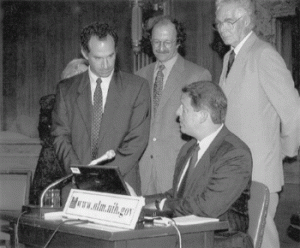
\includegraphics[width=4.00cm]{img/al-gore-pubmed-300x248.png}
\end{minipage}

\textbf{\large Who can participate in PubMed Commons at this time?}
\begin{itemize}
	\item Recipients of NIH (US) or Wellcome Trust (UK) grants can go to the NCBI website and register. You need a MyNCBI account, but they are available to the general public.
	\item If you are not a NIH or Wellcome Trust grant recipient, you are still eligible to participate if you are listed as an author on any publication listed in PubMed, even a letter to the editor. But you will need to be invited by somebody already signed up for participation in PubMed Commons. So, if you have a qualifying publication, you can simply get a colleague with the grant to sign up and then invite you.
\end{itemize} ~\\

\textbf{\large Inadequacies of letters to the editor as post-publication commentary~}~\\

Up until now, the main option for post publication commentary has been in later reviews of the literature, although there was a misplaced confidence in the more immediate letters to the editor. ~\\

\begin{minipage}[h]{4.25cm}
	
\includegraphics[width=4.00cm]{img/letter-to-editor-scaled500-300x217.png}
\end{minipage} \hfill \begin{minipage}[h]{14.75cm}
	I regret my \texttt{blog post last year~\footnotemark } recommending writing conventional letters to the editor. Letters remain \texttt{better than journal clubs~\footnotemark } for junior investigators eager to develop critical appraisal skills. But it could be a waste of time to send the letters off because letters are simply not effective contributions to post publication commentary. Letters never worked reliably well, and for a number reasons, they are now obsolete. ~\\
\end{minipage} ~\\
\footnotetext[1]{\texttt{http://jcoynester.wordpress.com/2012/02/08/why-you-should-write-letters-to-journal-edito/}}
\footnotetext[2]{\texttt{http://www.ingentaconnect.com/content/asahp/jah/2007/00000036/00000001/art00008}}

\begin{minipage}[h]{13.75cm}
	In the not-so-good-old days of exclusively print journals, there was a rationale for these journals putting limits on letters to the editor.
	\begin{itemize}
		\item With delays in availability due to the scheduling of print journals, letters to the editor were seldom available in a timely fashion. Readers usually would have long forgotten the article being critiqued when the letter finally came out.
		\item With limits on the number of pages allowed for issue, letters to the editor consumed a scarce resource without contributing to the impact factor of the Journal. So, journals typically had strict restrictions on the length of letters (usually 400 to 800 words), and a tight deadline to submit a letter after publication of the print article, usually no more than three months or less.
	\end{itemize} ~\\
\end{minipage} \hfill \begin{minipage}[h]{5.25cm}
	
\includegraphics[width=5.00cm]{img/hammering3pg.jpg}
\end{minipage}

\textbf{\large Editorial Review of letters to editor has seldom been fair.}
\begin{itemize}
	\item There is a prejudice against accepting anything but the most vitally relevant commentary. Yet editors are adverse to accepting critical letters that reflect badly on their own review processes. Get past the significance criterion and then you still risk offending the editor's sense of privilege.
	\item While letters to the editor are subject to peer review, responses from authors generally are not. Authors are free to dismiss or distort any criticism of their work, sometimes with the most absurd of statements going unchallenged.
	\item Electronic bibliographic resources have become the principal means of accessing articles, but no links are often provided between a letter to the editor and the target article. So, even if the credibility of the published article with thoroughly demolished in a letter to the editor, readers accessing that article through electronic bibliographic source are not informed.
	\item Many journals allowed authors to veto publication of any criticism of their work, but the journals do not state this in their instructions to authors. You can submit a letter to the editor, only to have it rejected because the author objects to what you said. But you are told nothing except that you letter is rejected.
	\item Many journals allow authors of the target articles the last word in responding to critical letters. Publishing a single letter and a response typically completes discussion of a target article. And the letter writer never gets to see the author's response until after it is published. So, you can put incredible effort into carefully expressing your points within the limits of 400 to 800 words, only to be made to look ridiculous with mischaracterizations you can do nothing about.
\end{itemize} %% ~\\

Letters to the editor are thus usually untimely, overly short, and inadequately referenced. And they elicit inadequate and even hostile responses from authors, but are generally ignored by everybody else. --- Letters to the editor are seldom cited and this is just one reflection of their failing to play a major role in moving the scientific discussion forward. ~\\

The advent of web-based publishing made restrictions on letters to the editor less justifiable. Once a basic structure for processing and posting letters to the editor is set up, processing and posting cost little. --- Print journals can reduce costs by maintaining a separate web-based place for letters to the editor, but restrictions on length and time to response have nonetheless continued, even if their economic justification has been lost. ~\\

\begin{minipage}[h]{14.75cm}
	BMJ Rapid Responses provides an exceptional model for post publication peer commentary. BMJ accepts electronic responses that can be accessed by readers within 72 hours, as long as the responses are not grossly irrelevant or libelous. Readers can register ``likes'' of Rapid Responses and threads of comments often develop. Then, a few comments are selected each week for editing and published in the print edition. Unfortunately, the rapid responses that remain only electronic are not indexed at PubMed and can only be found by going to the BMJ website, which is behind a pay wall for most articles. ~\\
\end{minipage} \hfill \begin{minipage}[h]{4.25cm}
	
\includegraphics[width=4.00cm]{img/bmj-logo-og.jpg}
\end{minipage}

Other journals are scrambling to copy and improve upon the BMJ model, but it can take some serious modification of software and that takes time. ``Like turning the Titanic around'' an editor of one of the largest open access journals told me. ~\\

\begin{minipage}[h]{6.25cm}
	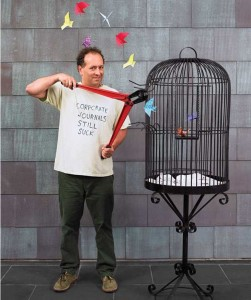
\includegraphics[width=6.00cm]{img/eisen_630-251x300.jpg}~\\
	\emph{\small PLOS cofounder Michael Eisen Photo by Andy Reynolds from Mother Jones}
\end{minipage} \hfill \begin{minipage}[h]{12.75cm}
	Until such options become widely available, a reluctance to writing letters to the editor remains thoroughly justifiable. Few letters will be submitted and fewer will be published or result in a genuine scientific exchange. And the goal remains elusive of readily accessible, indexed, citable letters to the editor and comments for which writers can gain academic credit. ~\\
	
	That is, unless PubMed Commons catches on.  It provides a potential of realizing PLOS Co-founder and disruptive innovator Michael Eisen's goal of continuous peer assessment and reassessment, not stopping with two or three people making an unreliable, but largely irreversible judgment that something should have been published and should eternally be accepted as peer-reviewed. ~\\
	
	PubMed Commons is only a rung on the ladder towards overthrowing the now firm line between publication and peer assessment. It's not a place to stop, but in important step. Please join in and help make it work. If you've ever publish an article listed in PubMed, find a way to get invited. If you not ready to post your own comments, lurk, offer others encouragement with ``like's'', and then when the spirit moves you, jump in! ~\\
\end{minipage}

I expect that someday soon you'll be a say to more junior colleagues, ``I was active in the field when authors could prevent you from commenting on their work and editors could prevent you from embarrassing them with demonstration of the stupidity of some of their decisions.'' And you junior colleagues can respond ``wow, was that in the days before email? Just how did you participate in the dialogue that is at the heart of scientific communication back then? Did you have to get up and challenge speakers at conferences?'' ~\\

\begin{center}
	\hfill \begin{minipage}[h]{2.25cm}
		
\includegraphics[width=2.00cm]{img/88x31.png}
	\end{minipage} \hfill \begin{minipage}[h]{10.00cm}
		Creative Commons License	
		\emph{\small This work, unless otherwise expressly stated, is licensed under a Creative Commons Attribution 3.0 Unported License. }
	\end{minipage} \hfill 
\end{center}

{\small 
	\textbf{About James Coyne PhD} %% ~\\

	James C. Coyne, Ph.D. is Professor of Psychology in the Department of Psychiatry, Director, Behavioral Oncology Research of the Abramson Cancer Center, and a Senior Fellow at the Leonard Davis Institute for Health Economics, all at the Perelman Medical School of University of Pennsylvania. Additionally, he is Professor of Health Psychology, University of Groningen Medical Center (UMCG), the Netherlands. Previously, he served on the faculties of University of California, Berkeley and University of Michigan School of Medicine. Dr. Coyne has been elected a Fellow of the American Psychological Association, Society of Behavioral Medicine, and Academy of Behavioral Medicine. His critical commentaries have challenged whether psychosocial intervention extends the survival of cancer patients, whether recommended and mandated depression programs improve patient outcomes, and whether meta analyses of behavioral medicine commissioned by professional organizations are valid and credible. A 2008 systematic review and meta-analysis in JAMA of screening for depression among cardiovascular patients was designated by BMJ as one of the eight top papers of the year. He is known for presenting and defending controversial positions and for promoting reform of the clinical and health psychology journals. He is the co-author or editor of a number of books including the 2009 Screening for Depression in Clinical Settings: An Evidence-Based Review (Oxford University Press) with Alex Mitchell. ~\\
} %% \small

\end{document}
